\section{Code implementation}
\label{sec:codeimpl}

	\subsection{MATLAB environment}
		As mentioned on chapter \ref{ch:setup}, FLIR software provides indexed matrices in .mat format to be used directly in MATLAB. Each pixel contains the temperature information about that location in the picture. It is possible to visualize an example of a scaled image on the following figure:

		\begin{figure}[H]
			\centering
			\captionsetup{justification=centering}
			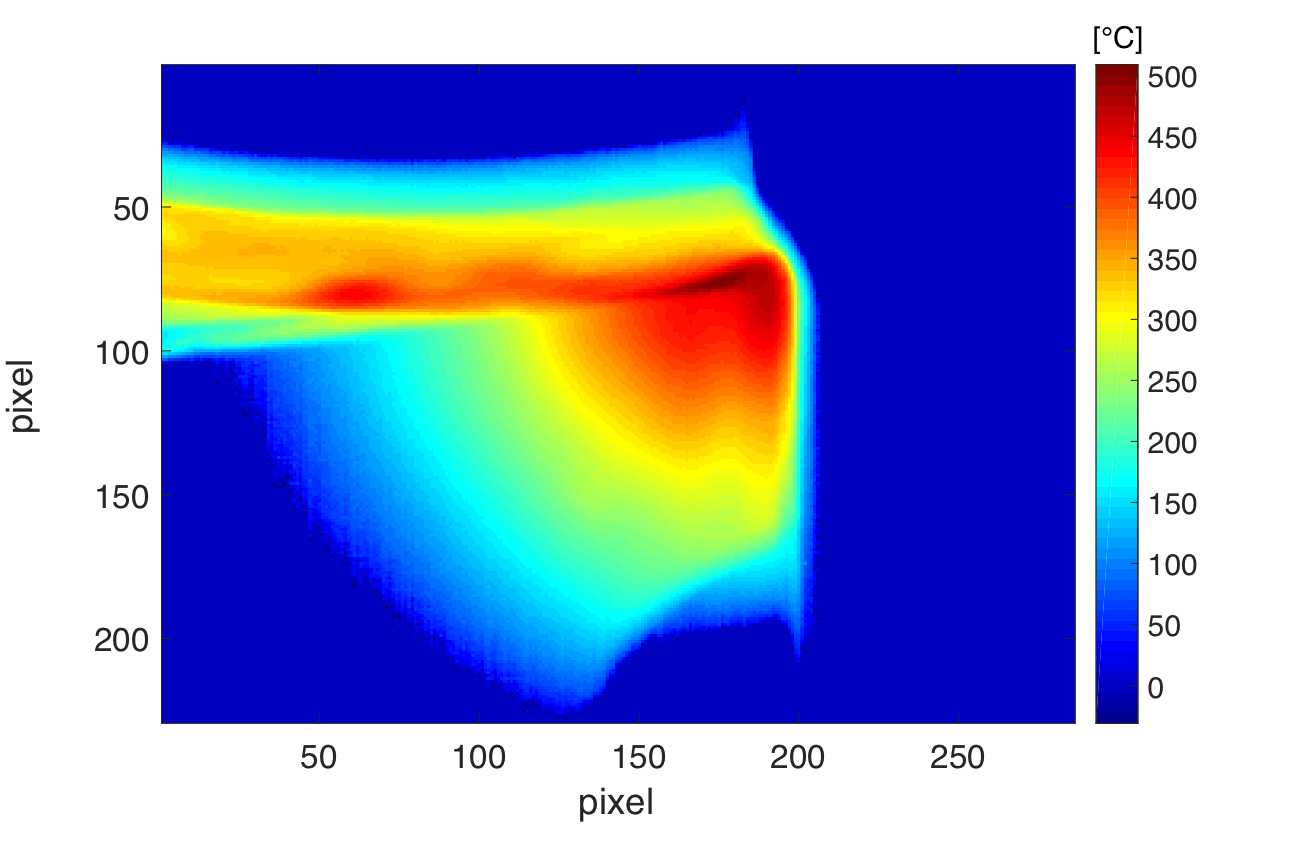
\includegraphics[scale=0.6]{Cap4/TempDist.png}
			\caption{Thermal image for $t_{uc} = 200\mu m$ and $v_{c} = 100 m/min$ scaled in MATLAB}
			\label{fig:tempdist}
		\end{figure}

		From figure \ref{fig:tempdist} and with MATLAB Image Processing Toolbox support it was possible to extract features that will futher help to capture the behavior of heat flows and heat partitions. They are:

		\begin{itemize}
			\item Rake and clearance face recognition
			\item Detection of tool tip
			\item Image segmentation of tool, chip and workpiece
			\item Isotherm coordinates along tool shape
		\end{itemize}
	
	\subsection{Auxiliary functions}

		Some functions used to build the method were already implemented in MATLAB's library. To understand the output of these functions, the next subsections will present their operation and final aim.

		\subsubsection{Contour plot}
		\label{ch:seccontour}
			An important tool for the development of the method, contour plot is able to provide same level curves. Since the basic variable provided is the temperature along cutting zone, this function will calculate continuous lines of very close values of temperature. Doing it with a small tolerance, the lines calculated will be the corresponding isotherms of the image. Hence, it is easier to extract the coordinates of each pixel in these lines for each level of temperature.

			\begin{figure}[H]
				\centering
				\captionsetup{justification=centering}
				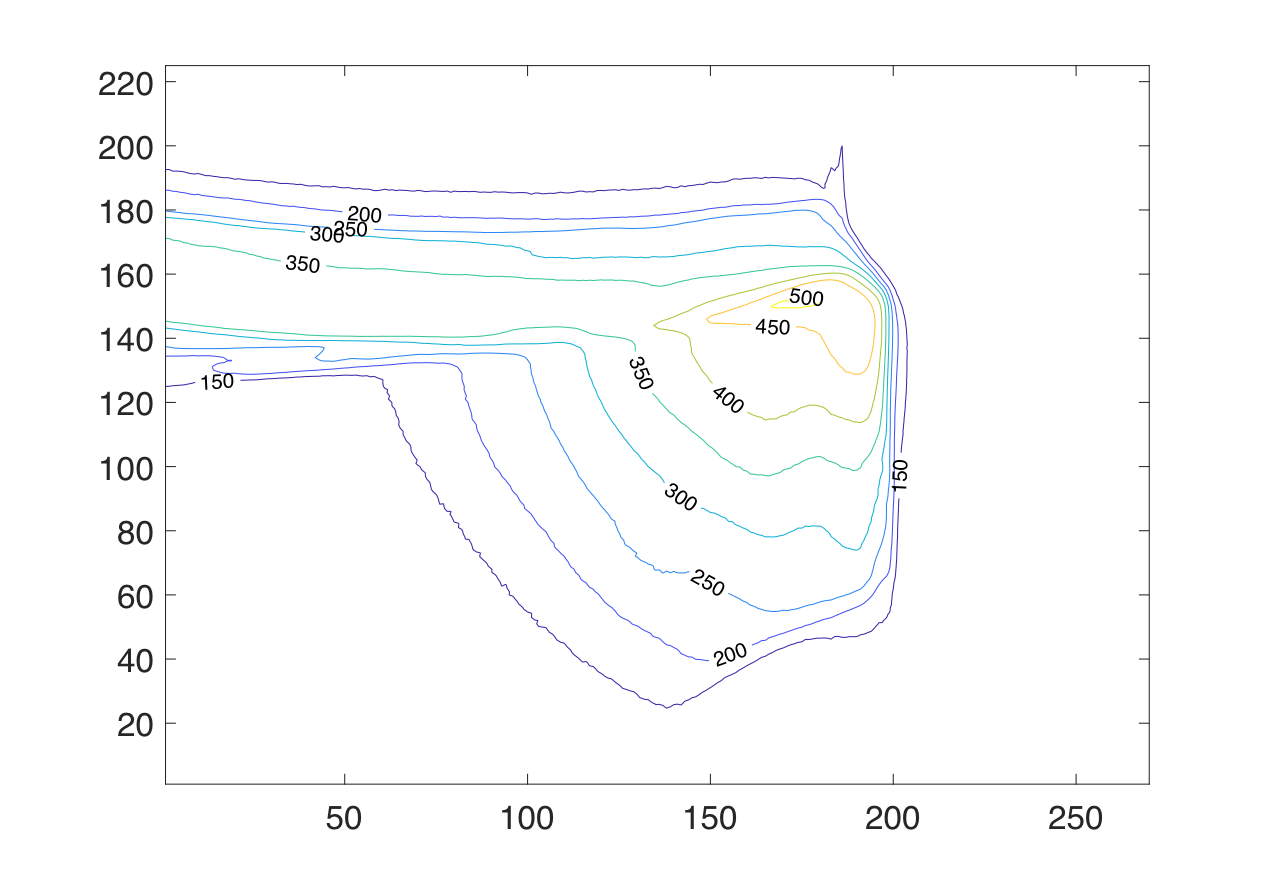
\includegraphics[scale=0.6]{Cap4/contour.png}
				\caption{Contour plot for $t_{uc} = 200\mu m$ and $v_{c} = 100 m/min$}
				\label{fig:contour}
			\end{figure}

		\subsubsection{Hough lines transformation}
		\label{ch:sechough}
			Hough transform is an extensive method used in computer vision. It is an extraction feature for complex geometries, using normal parameterization for straight lines \cite{duda1972use}. In MATLAB, the parametric equation of the lines is stated in equation \ref{eq_parametric}.

			\begin{figure}[H]
				\centering
				\captionsetup{justification=centering}
				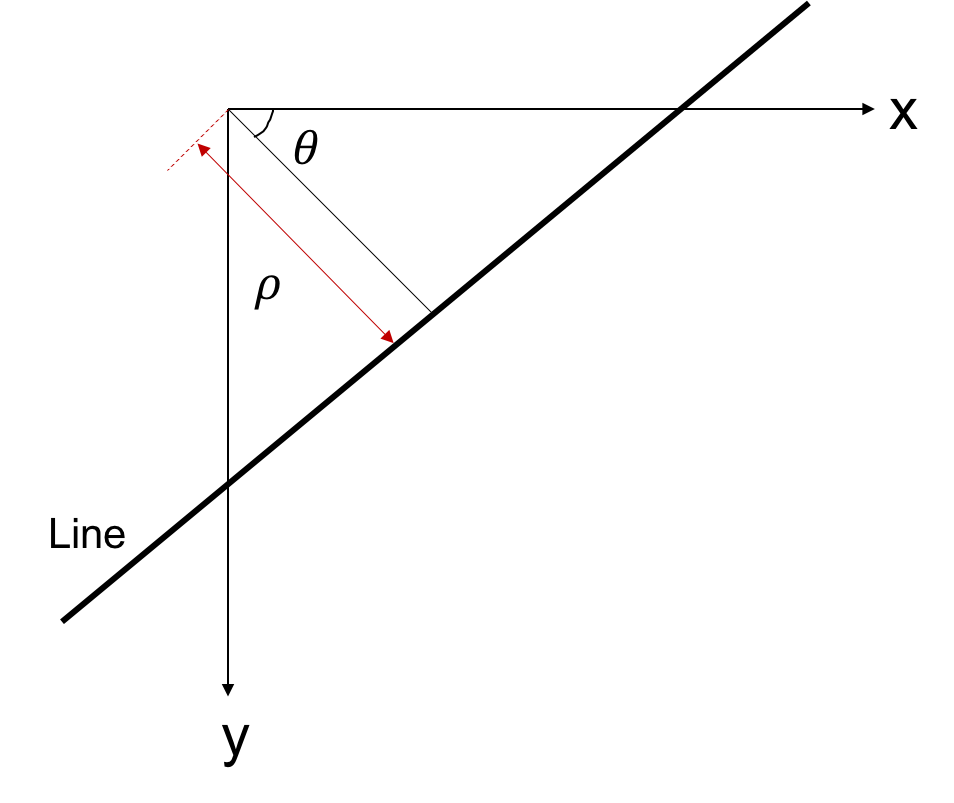
\includegraphics[scale = 0.5]{Imagens/houghp.png}
				\caption{Reference for hough parametrization (Source: Mathworks)}
				\label{fig:houghp}
			\end{figure}

			\begin{equation} 
			\label{eq_parametric}
			\rho = x\times cos(\theta) + y\times sin(\theta)
			\end{equation}

			Concerning the images, the rake and clearance face can be mapped by means of hough lines transformation in MATLAB. It is necessary to provide a probable range of angles in which the angular coefficient of the sought lines is defined. The more precise is this range, more reliable and faster will be the output.			

			\begin{figure}[H]
				\centering
				\captionsetup{justification=centering}
				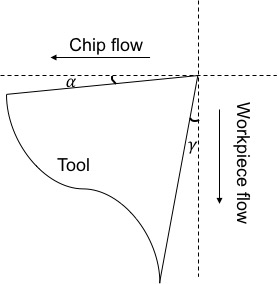
\includegraphics[scale = 0.65]{Cap4/imgset.jpg}
				\caption{Placement of tool}
				\label{fig:imgset}
			\end{figure}

			The test bench, where the experiments were performed, allows for a fixed positioning of the tool in relation to the thermal camera. It means that the angle between the rake face and horizontal line and the angle between clearance face and vertical line are always the designed rake and clearance angles, respectively. In other words, the tool does not rotate in relation to the reference axes. Because of this, it is possible to perform hough transformation on the image, with very high accuracy. However, sometimes the chip can cause interference on the measurements of the edges, making the feature extraction impractical.

	\subsection{Implementation steps}

		This subsection will present an overview of the code implementation and the logical sequence of what was implemented, showing each step taken to develop the next one. The steps that will be presented represent the key path for the code development.

		\subsubsection{Overview}	

			The program was able to identify tool and chip shapes, allowing the image segmentation of the components and, consequently, the thermal analysis of each part separately. By means of image processing and input data about cutting parameters, features like maximum temperature in the cutting zone, maximum chip temperature, heat flow through chip and tool are some examples of what the code is able to provide.	
			
		\subsubsection{Finding tool edges}

			As mentioned in the subsection \nameref{ch:sechough}, the Hough transform was essential to detect edges. In order to make the code faster, the edges of the original thermal image were extracted, creating a binary image (figure \ref{fig:edges}).

			\begin{figure}[H]
			\centering
			\captionsetup{justification=centering}
			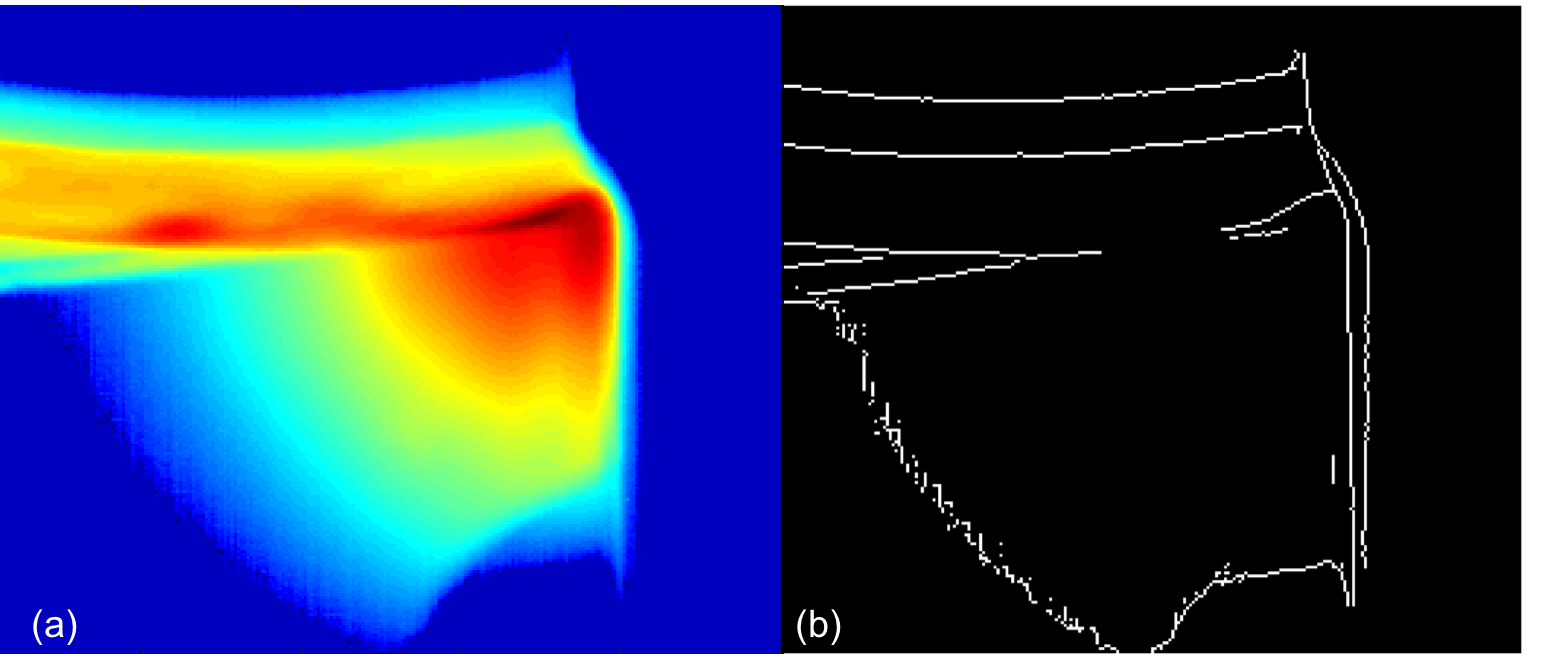
\includegraphics[scale = 0.5]{Imagens/edges.png}
			\caption{(a) Original thermal image and (b) Edges detected by MATLAB}
			\label{fig:edges}
			\end{figure}

			Given the previous figure, the hough transform is applied directly on the binary image, which only has information about the edges. Because of it, the hough transform performance is faster than it would if applied to the original image. The source code for hough implementation is showed on the following script:

			\lstinputlisting[firstline=282,lastline=329]{ApeA/TemperatureAnalyze.m}

			Since the rake angle is $6^{o}$ and the clearance angle is $3^{o}$, ranges of [81:85] and [2:5] were given to each one respectively, as it can be observed on lines 4 and 20. Regarding the rake angle, the range of angles is given by the complementary operation due to the reference in hough method. This way, the hough transform returns highlighted points in the accumulation matrix of hough process and from them the 10 first points are chosen to be analyzed, which is a reasonable amount of points which may represent sections of the rake and clearance lines.

			The fixed position of the tool also allows the predetermination of the $\rho$ parameter, which is the distance of the detected lines from the reference in hough. This is also seen on lines 14 and 30 as boundary conditions to determine the right edge lines. The outputs of this function are the extremity coordinates of the detected line and also the angle of the corresponding angular coefficient. 

			Sometimes it was necessary to set default conditions, as rake and clearance angles, due to chip obstruction. The chip obstruction causes interference on the temperature fields, which can disturb the edges definition in thermal images, preventing the proper functioning of hough transform.

		\subsubsection{Rake and clearance face}

			With the data provided by the output of the hough function, the equation that defines each straight line corresponding to the edges is known. So, it is possible to extend the lines to match the entire rake and clearance edges.

			\begin{figure}[H]
			\centering
			\captionsetup{justification=centering}
			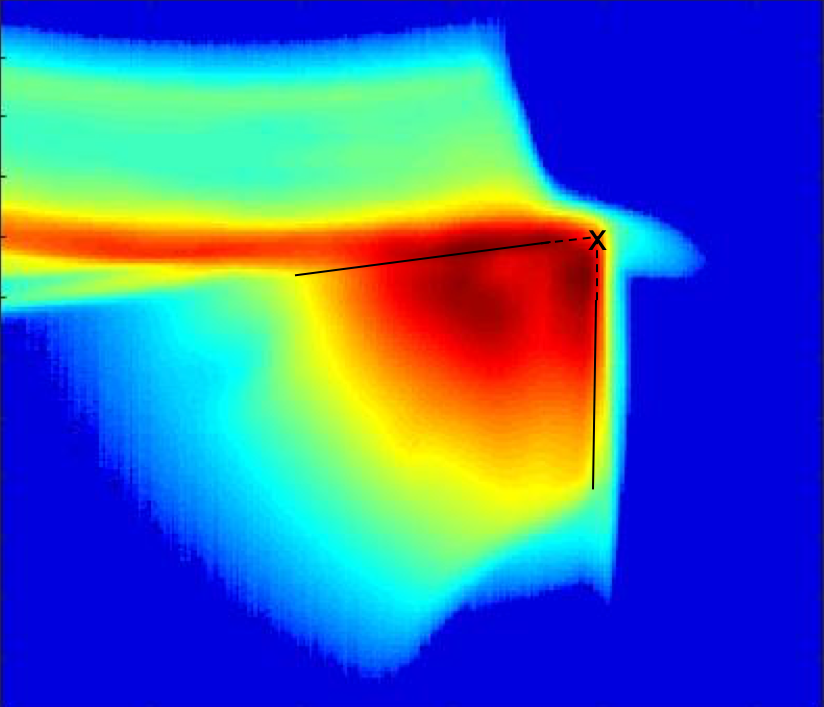
\includegraphics[scale = 0.6]{Imagens/hough.png}
			\caption{Lines detected by hough transformation method}
			\label{fig:hough}
			\end{figure}

			This is an important step of the method because it allows to build a mask (figure \ref{fig:mask}), which is a binary image with the tool shape, that is able to remove only the region of interest. Consequently, it will be possible to analyze the temperature fields and thermal behavior inside the tool without any interference from the temperatures in the vicinity.

			\begin{figure}[H]
			\centering
			\captionsetup{justification=centering}
			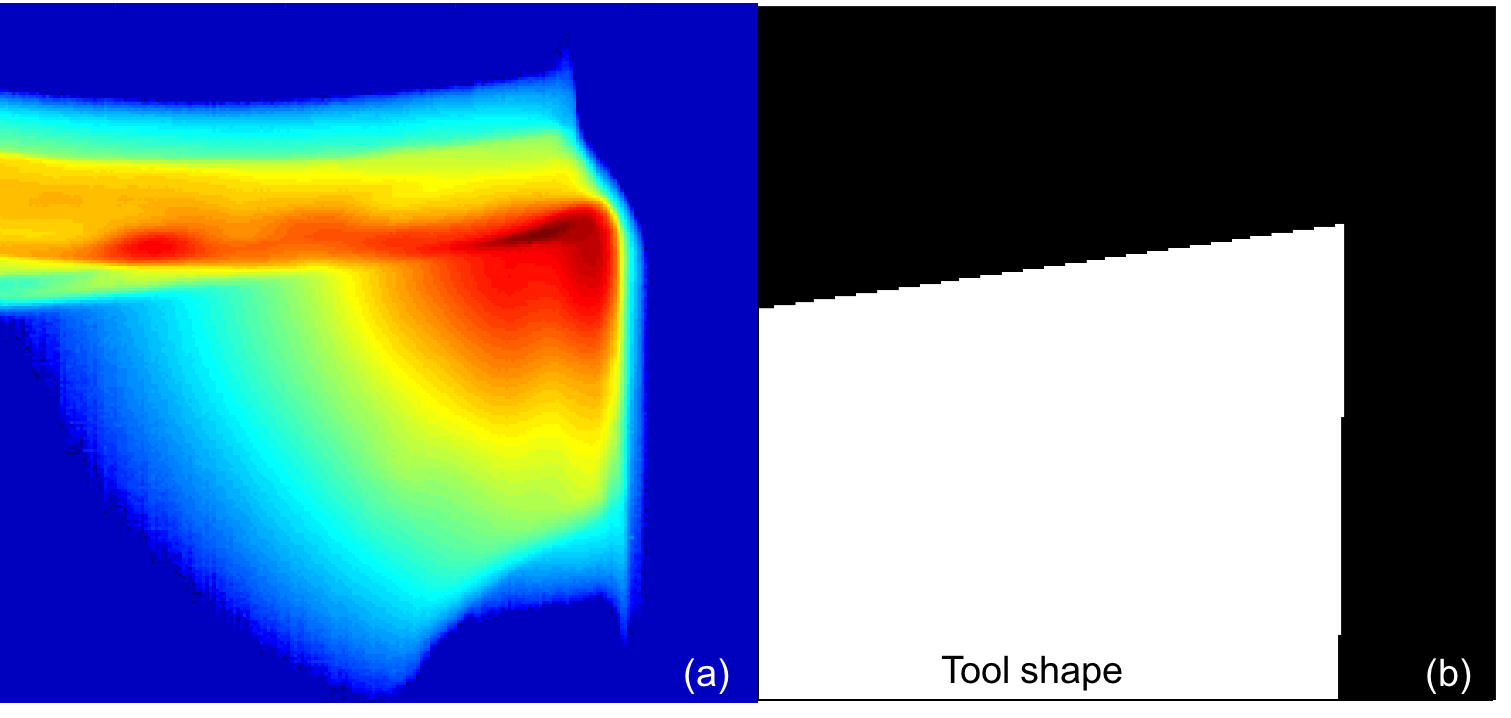
\includegraphics[scale = 0.5]{Imagens/mask.png}
			\caption{(a) Original image and (b) Region of interest - tool}
			\label{fig:mask}
			\end{figure}

		\subsubsection{Tool tip coordinates}

			As the rake and clearance edges are determined, the tool tip is calculated by means of the intersection between these lines. On the figure \ref{fig:hough}, the found lines are extended until they intersect, then the tool tip coordinates can be calculated. It is important to determine these coordinates due to the interest in knowing the temperatures of the area close to the tip and what is the maximum value it can reach, which is related directly with tool life and therefore the surface finish.

		\subsubsection{Maximum temperatures}

			Since the code was able to segment the tool shape from the entire matrix, it gets easier to extract the chip contour, which is the other region of interest which presents measurable range of temperatures. Getting the maximum temperature from each zone allows not only to know if the measured temperatures are inside the measurement limit, but also to compare the behavior of this maximum temperature for different cutting velocities and depths of cut.

			The maximum temperature in the cutting zone raises as the cutting process happens (figure \ref{fig:maxtemp}). For a same value of underformed chip thickness, the higher is the cutting velocity the lower will be the value of maximum temperature reached.

			\begin{figure}[H]
			\centering
			\captionsetup{justification=centering}
			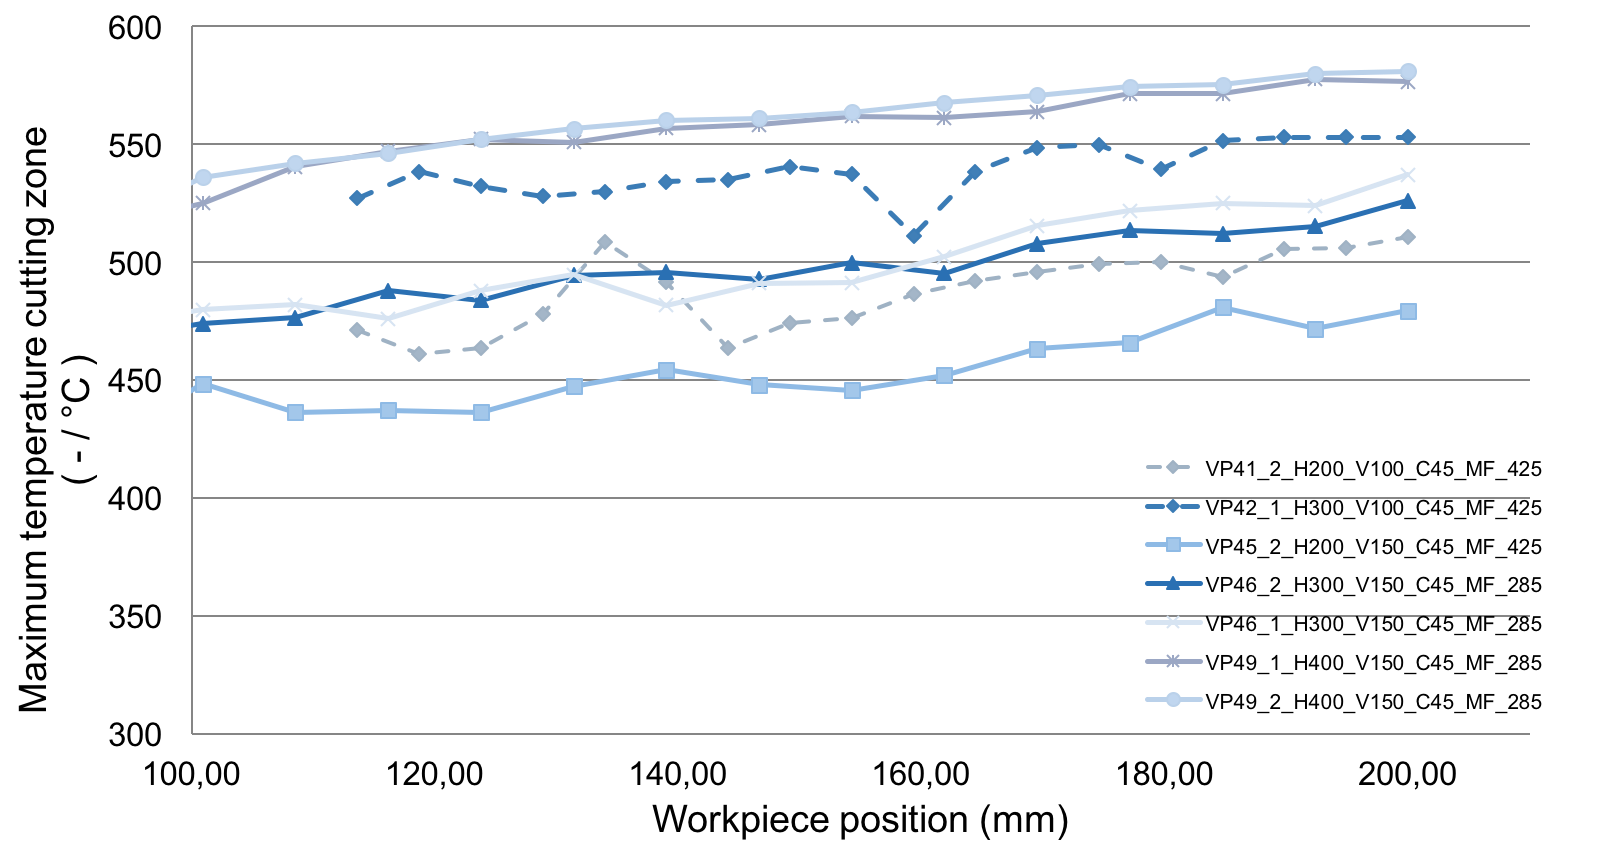
\includegraphics[scale = 0.55]{Imagens/maxtemp.png}
			\caption{Maximum temperature of the cutting for the designed experiments}
			\label{fig:maxtemp}
			\end{figure}

		\subsubsection{Temperature fields}

			In this step, the auxiliary function will be used mentioned on the subsection \nameref{ch:seccontour}. For the application in this method, a step of 40$^{o}C$ was taken to separate each level of temperature. The use of the function is simple, being necessary only to provide the image (\texttt{obj.frame}) and the spacing vector between levels (\texttt{v}).

		
			\lstinputlisting[firstline=610,lastline=610]{ApeA/TemperatureAnalyze.m}

			The output of contour function is a matrix C with 2 rows that will provide the levels of temperature and the number of coordinates followed by their absolute values of \texttt{x} and \texttt{y}, providing the location of each point of the isothermal curves.

			\begin{mdframed}[backgroundcolor=lightgray!25!]
			\begin{alltt}\fontsize{9pt}{8pt}\fontfamily{pcr}\selectfont
			C    =  [C(1) C(2) C(3) ...C(k)... C(N)]
			C(k) =  [level x(1) x(2)...
			         numxy y(1) y(2)...]
			\end{alltt}
			\end{mdframed}
			
			For each matrix \texttt{C(k)}, \texttt{level} shows which temperature the following points are representing and \texttt{numxy} is the number of coordinates used to build the corresponding level. The coordinates are represented in the pair \texttt{(x,y)}.

			Also, it is possible to visualize the evolution of the isotherms and, consequently, the temperature gradients with contour plot. An example can be observed on figure \ref{fig:gradient}. The distance between the lines slightly increases as the cutting process advances. This points to a reduction of the gradient values, which indicates a negative rate of heat into the tool along the time.

			\begin{figure}[H]
			\centering
			\captionsetup{justification=centering}
			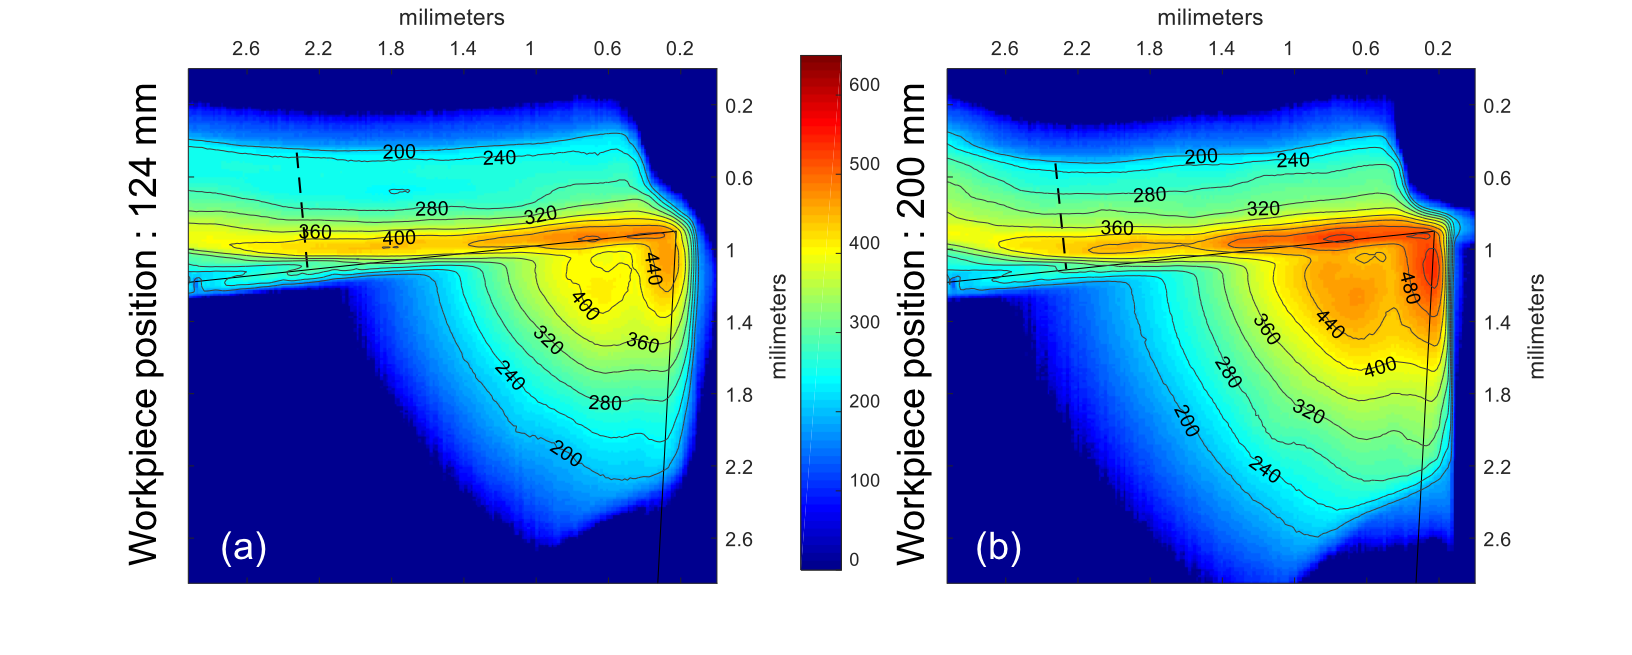
\includegraphics[scale = 0.6]{Imagens/gradient.png}
			\caption{(a) Temperature field for workpiece position 124 mm (b) Temperature field for workpiece position 200 mm}
			\label{fig:gradient}
			\end{figure}

		\subsubsection{Heat flows - Chip and Tool}
		\label{heatflows}

			As described on section \ref{methods}, the heat flow through the tool and the energy carried away by the chip are calculated. For heat flow through the tool, it is possible to extract isothermal lines by means of contour plot and to calculate the temperature gradient, which is already normal to the isothermal lines due to its properties. The tool width is already known (subsection \ref{sec:exSetup}). The length of the chosen isotherm is given by counting the amount of pixels in \texttt{numxy}, as described in the previous subsection, and then it is converted to millimeter with the scale factor.
			In the case of the energy carried away by chip, the chosen line is placed on the end of chip-tool contact, which is where the maximum temperature of the chip - tool interface occurs \cite{abukhshim2006heat}, \cite{boothroyd1963temperatures}. The explanation is that all the heat source in the friction zone is located before this line. In other words, there is no other heat source after this line that could provide more thermal energy to be carried away by chip.		

		\subsubsection{Heat partitions}

			Having the results of the subsection \ref{heatflows}, these values can be combined with the total power ($P$) generated during the cutting process (equation \ref{eq_power}) to calculate the energy that goes to the workpiece by means of energy balance (equation \ref{eq_energybalance}). Hence, it is possible to calculate the heat partition relative to each zone of interest.

			\begin{equation} 
			\label{eq_heatpartition}
			p_{i} = \frac{\dot{Q}_{i}}{P}
			\end{equation}

			Where the index $i$ is related to $C$ (chip), $W$ (workpiece) and $T$ (tool).

	\section{Method validation}

		As described along section \ref{sec:codeimpl}, there are many outputs from the implemented method, shear and normal stresses related to the mechanical part, for example. However, in this paper the heat partitions will be the focus of discussions.

		The total power produced along this high speed machining was calculated as in the equation \ref{eq_power}. The values are shown on figure \ref{fig:totPower}.

		\begin{figure}[H]
			\centering
			\captionsetup{justification=centering}
			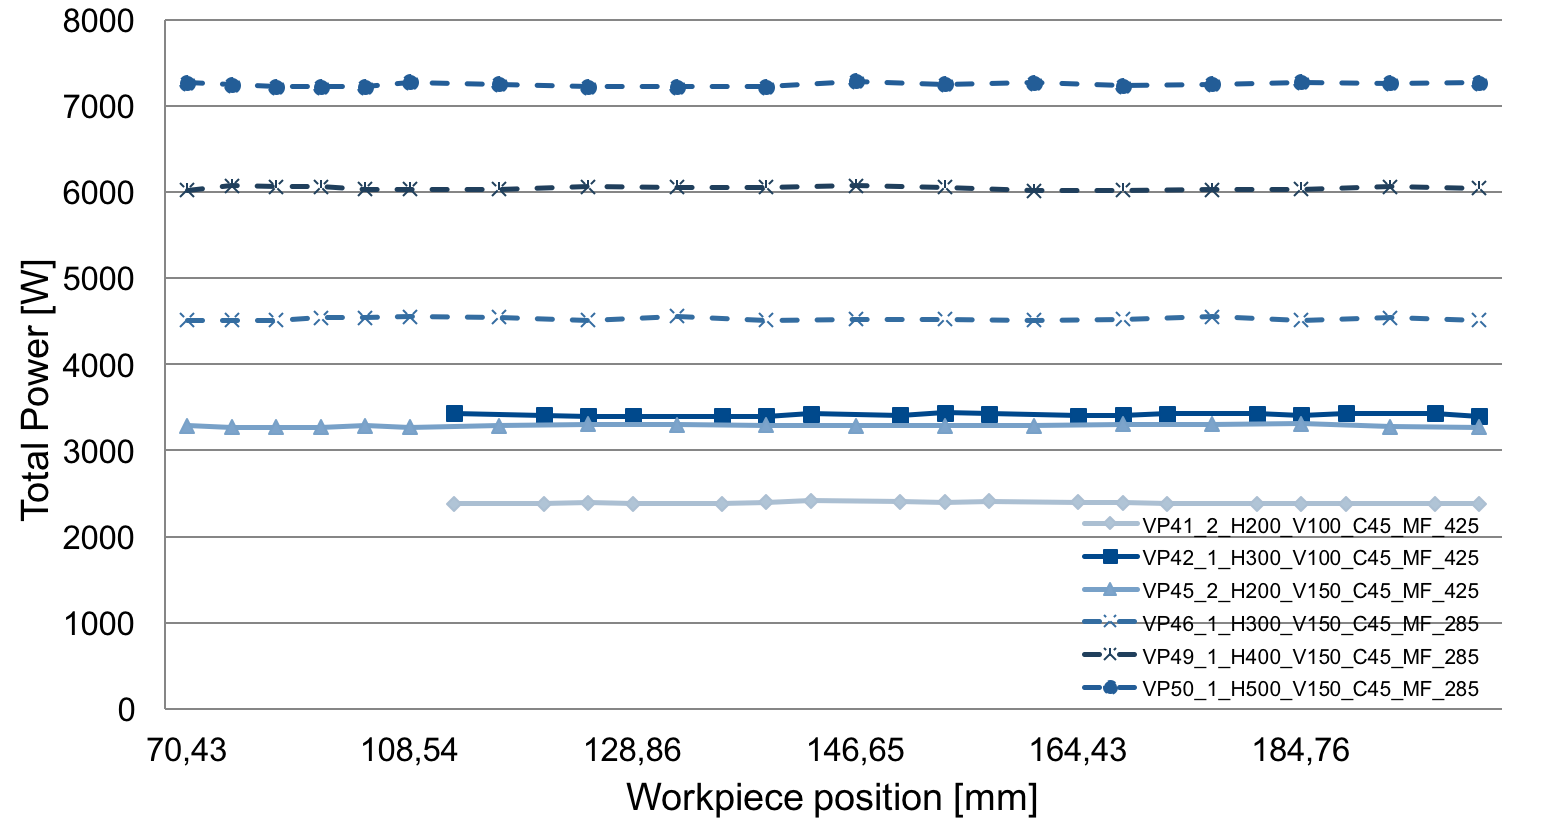
\includegraphics[scale=0.55]{Imagens/Total_power.png}
			\caption{Total power produced}
			\label{fig:totPower}
		\end{figure}

		As expected, the higher are the values for cutting velocity or depth of cut, higher are the values for total power produced.
		For each experiment, the computational method was able to provide the thermal energy that goes to tool, chip and workpiece by means of energy balance. Then, the thermal behavior of every area of interest along the workpiece position can be observed. The measurement starts when a reasonable area of the cutting zone reaches the minimum measurable temperature. For cutting velocity of $150 m/min$ it starts earlier because the rate of heat production is higher than when the cutting velocity is $100 m/min$.

		\begin{figure}[H]
			\centering
			\captionsetup{justification=centering}
			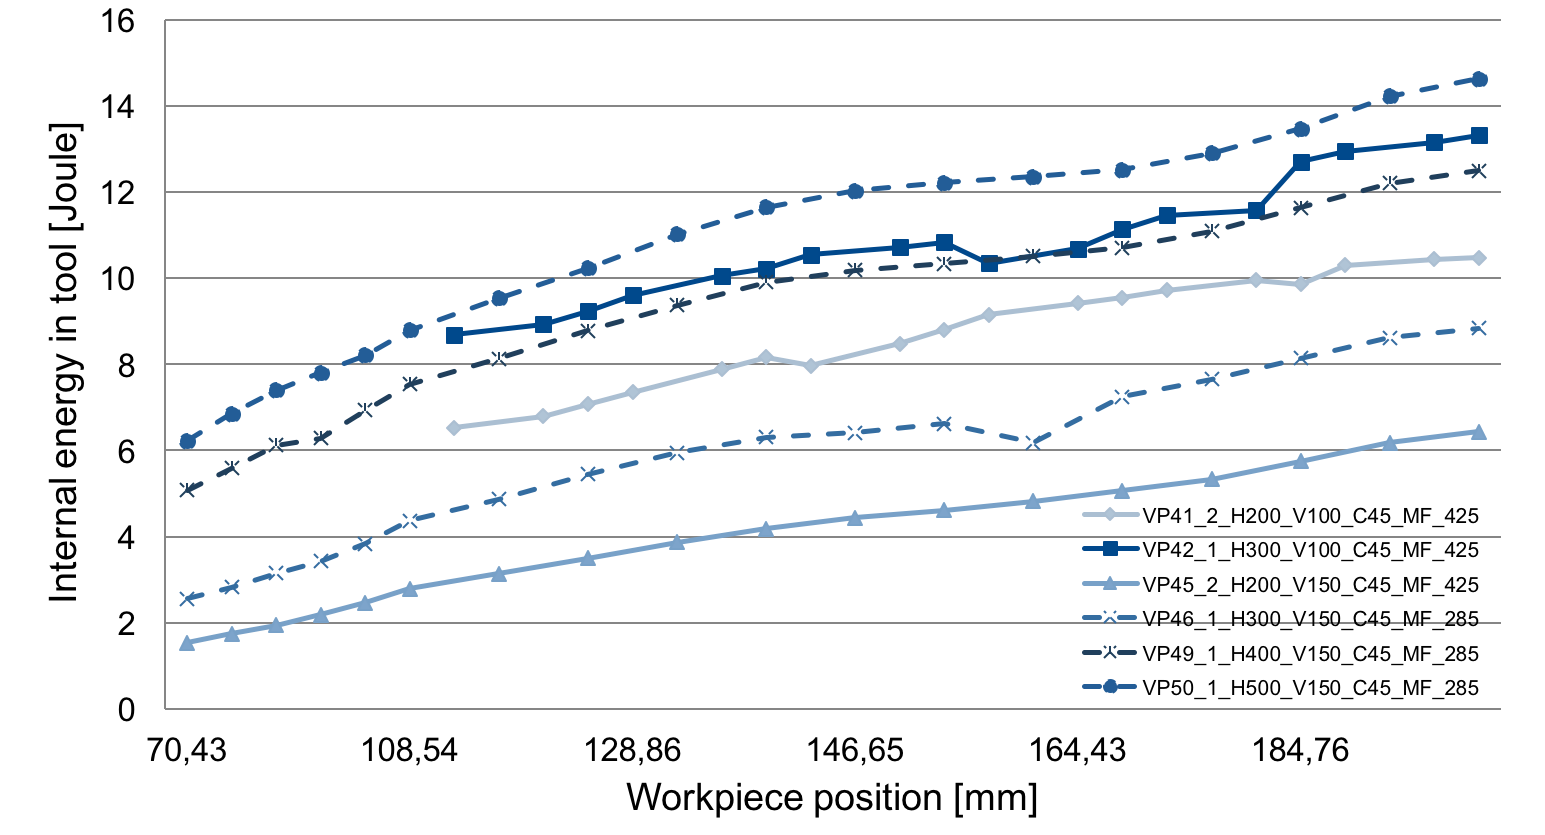
\includegraphics[scale=0.55]{Imagens/Inner_Energy.png}
			\caption{Inner energy of the tool along workpiece position}
			\label{fig:innerTool}
		\end{figure}

		\begin{figure}[H]
			\centering
			\captionsetup{justification=centering}
			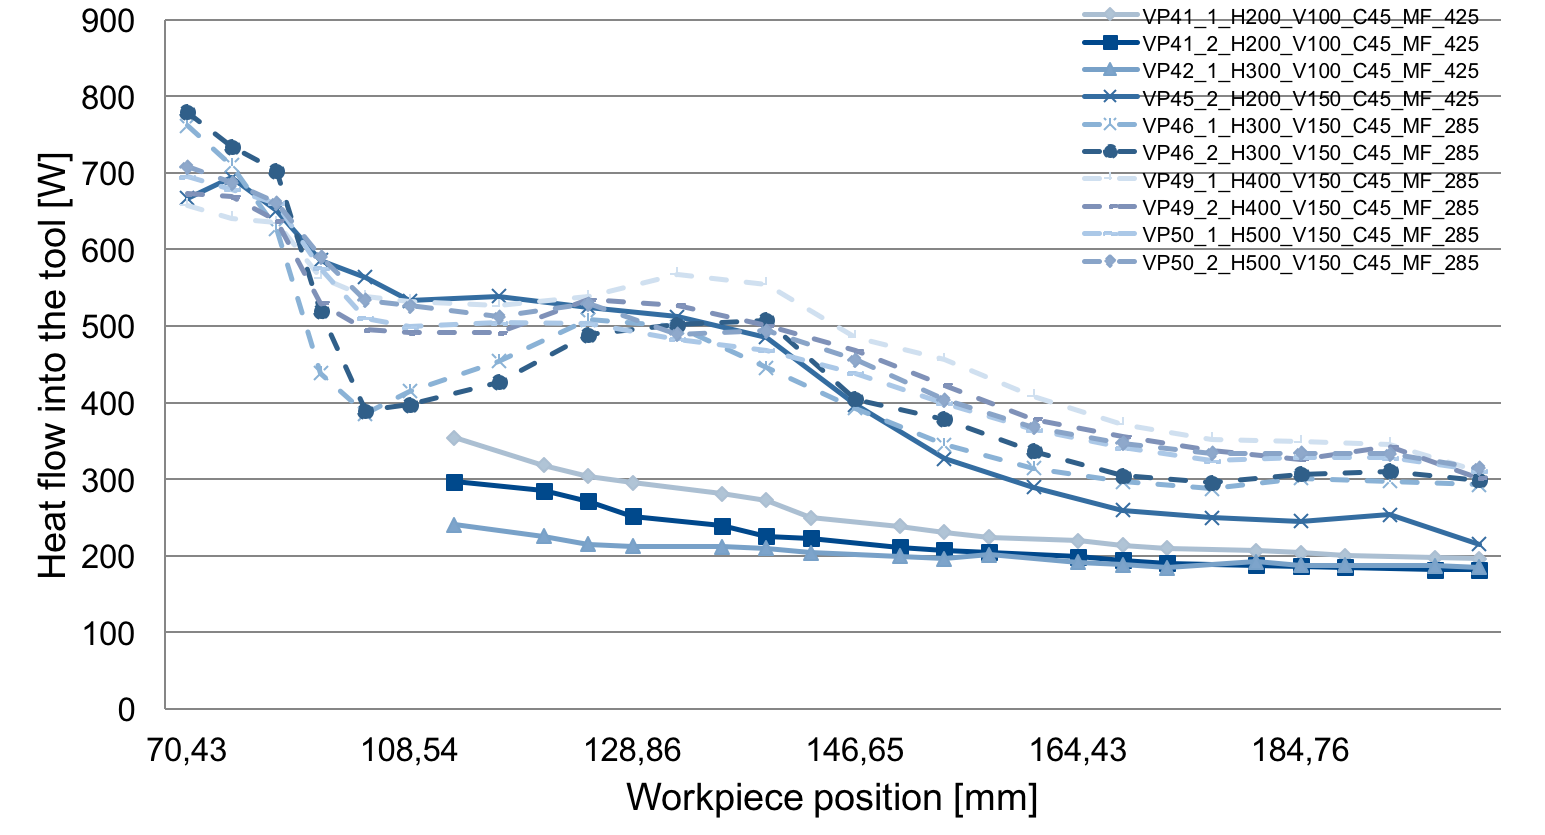
\includegraphics[scale=0.55]{Imagens/energyTool2.png}
			\caption{Heat flow into the tool}
			\label{fig:hflowTool}
		\end{figure}

		As it can be observed on the previous figure \ref{fig:hflowTool}, the change rate of the inner energy of the tool begins with a higher value than in the end of the process. The rate starts to stabilize, indicating the beginning of the steady state. 

		Still regarding the tool (figure \ref{fig:hpartTool}), the partition of energy can reach a range that goes from about 20\% in the transient state down to 4\% close to the end of the cutting process, where it reaches the steady state. \citeonline{takeuchi1982improvement} presents that 10 - 30\% of the total heat generated is removed through the tool, which is in agreement with the presented result.

		\begin{figure}[H]
			\centering
			\captionsetup{justification=centering}
			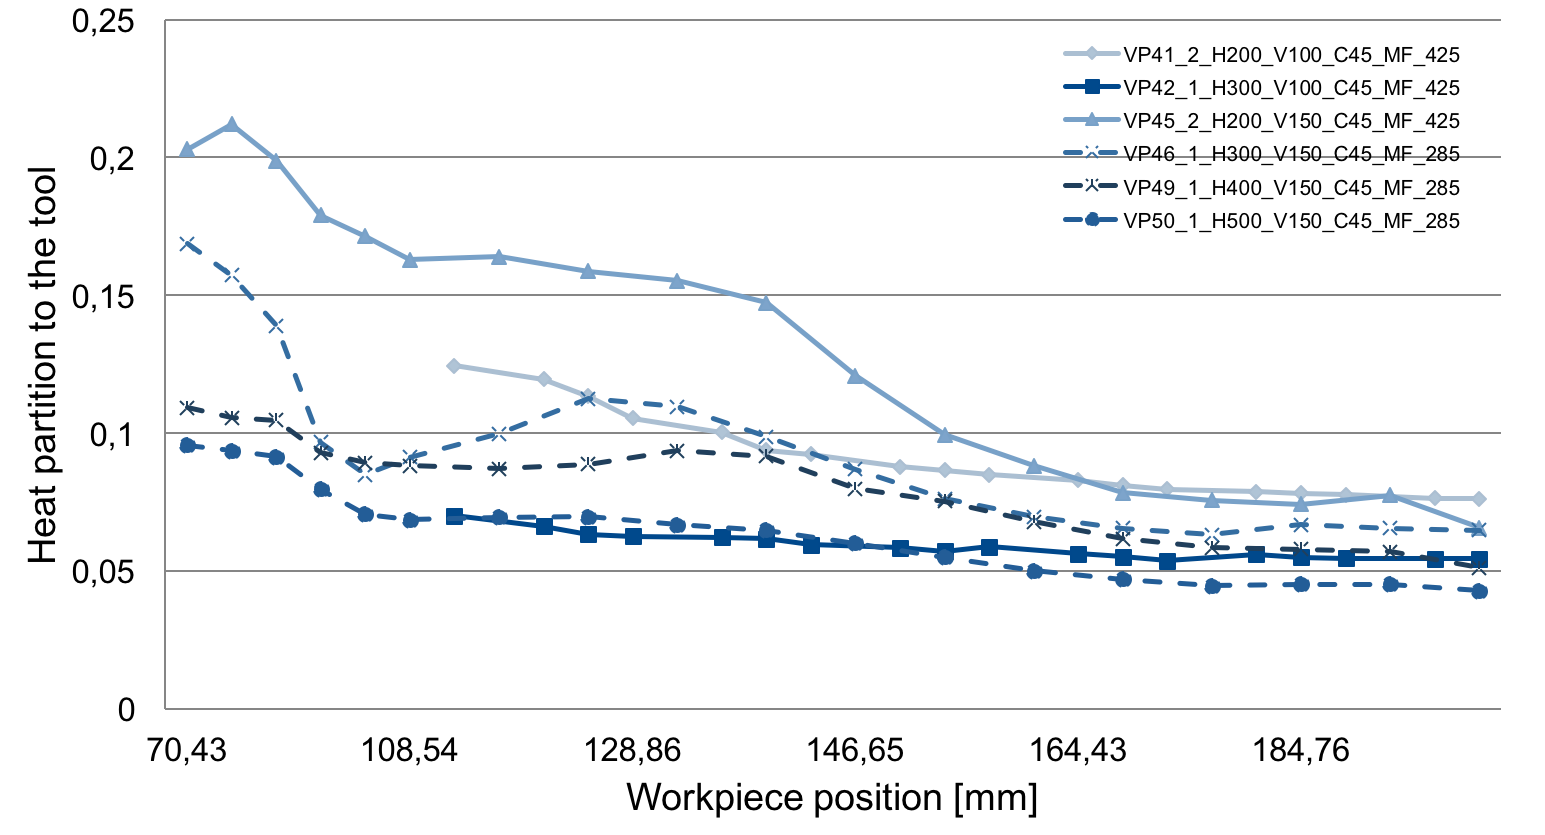
\includegraphics[scale=0.55]{Imagens/partTool.png}
			\caption{Heat partition ratio for the tool}
			\label{fig:hpartTool}
		\end{figure}

		Also \citeonline{augspurger2016modelling} proposed a model based on the use of Green's function for temperature prediction along the tool shape during transient state. The experiments were the same as the ones presented in this work. Using the same heat flow into the tool to simulate temperature fiels, the result showed a good approximation between model and experimental data.

		Regarding the chip, it is important to highlight the total power produced during the cutting process, which has a significant value because of the high values of cutting velocity and force. Moreover, it must be also noticed the amount of energy that goes to the chip (figure \ref{fig:energyChip} and \ref{fig:hpartChip}). The chip takes around 70\% of the total energy produced, which may be explained by the high temperatures that the region can reach and the high velocity of flowing.

		\begin{figure}[H]
			\centering
			\captionsetup{justification=centering}
			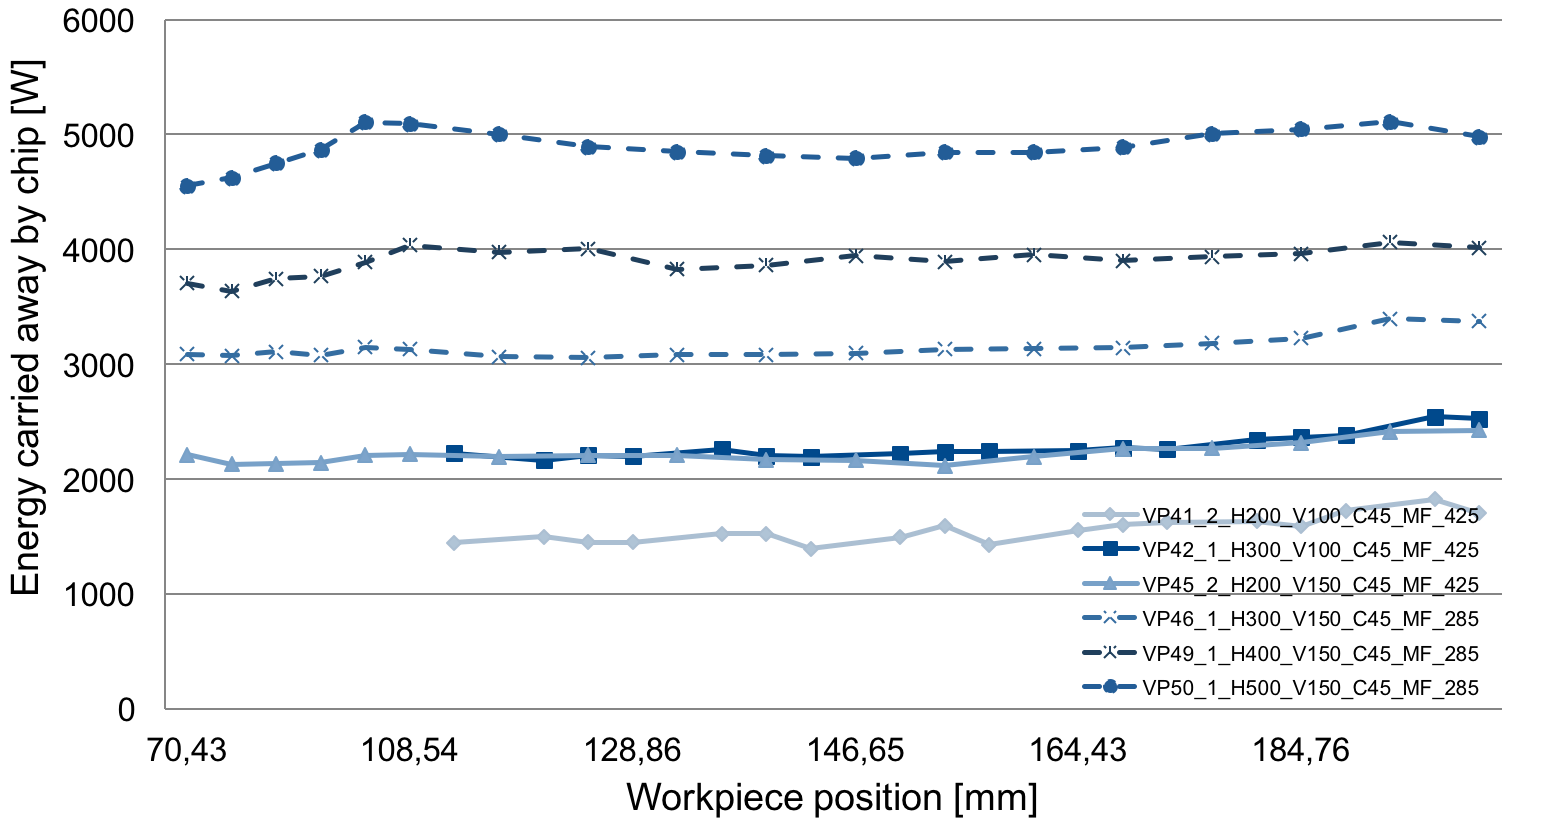
\includegraphics[scale=0.55]{Imagens/energyChip.png}
			\caption{Thermal energy into the chip}
			\label{fig:energyChip}
		\end{figure}

		\begin{figure}[H]
			\centering
			\captionsetup{justification=centering}
			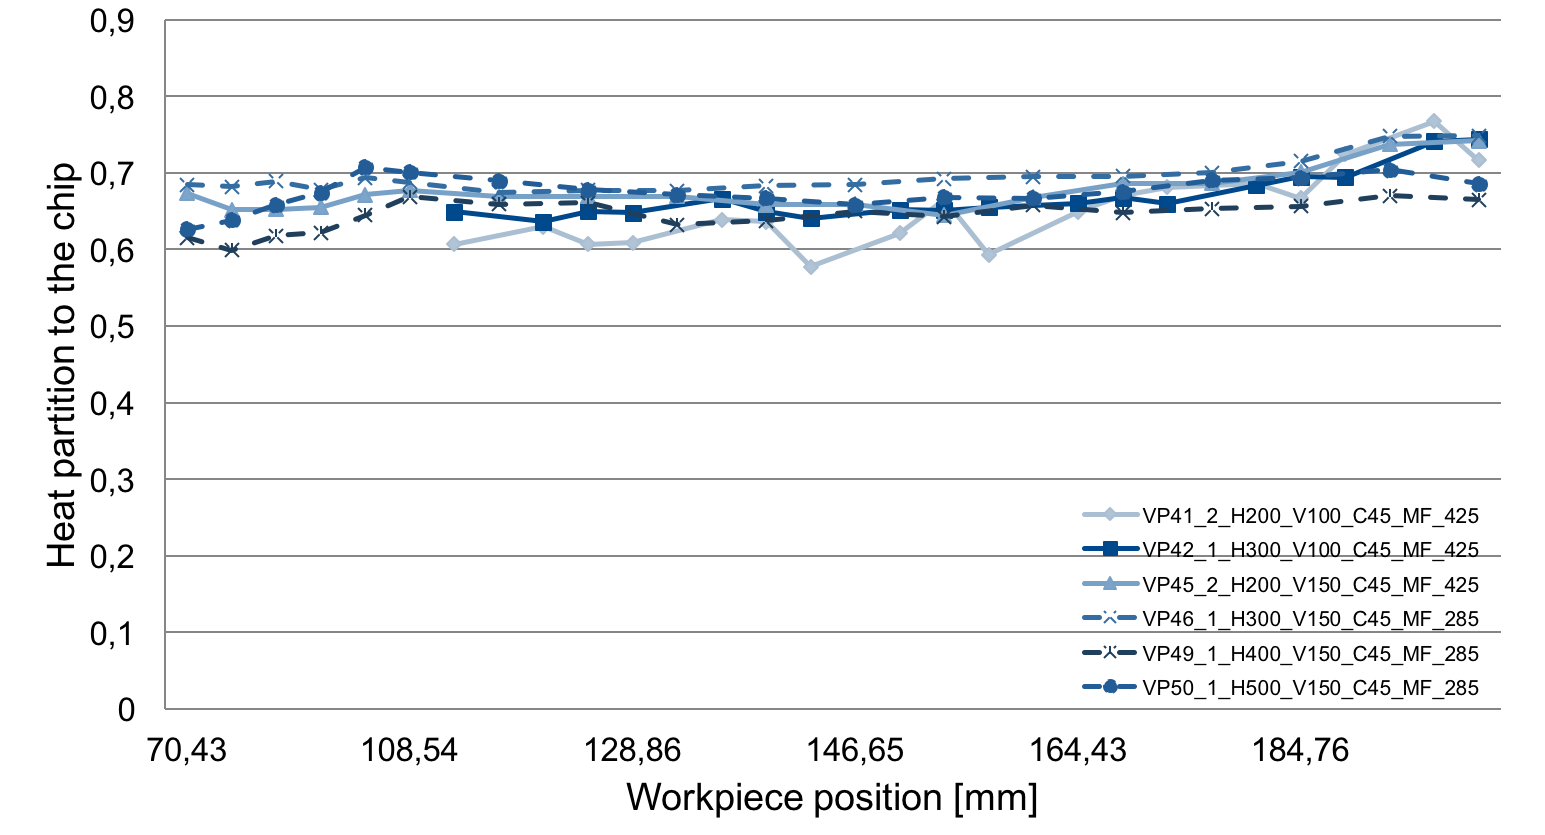
\includegraphics[scale=0.55]{Imagens/PartChip.png}
			\caption{Heat partition ratio for the chip}
			\label{fig:hpartChip}
		\end{figure}

		\citeonline{trigger1942} presented a model for the average temperature prediction in the cutting zone. The proposed model was made for steady state and the existence of only two heat sources was considered, the primary and secondary shear zones. The heat partitions were assumed as 90\% for the chip and 10\% for the tool. It is known that the tertiary zone has a minor influence on heat generation given the cutting conditions (subsection \ref{subsec:heatzones}) and, consequently, the temperature raise in the tool is mainly caused by the friction zone. Then, the heat partition about 70\% for the chip (figure \ref{fig:hpartChip}) and 6\% for the tool (figure \ref{fig:hpartTool}) in the steady state will represent around 92\% for the chip and 8\% for the tool of all heat produced in the primary and secondary shear zones. It agrees with the proposed assumption.

		It may be noticed that for experiments with the same relation $v_{c}\times a_{p}$ (figure \ref{fig:energyChip}) apparentely the same amount of energy is carried by the flowing chip. On the other hand, the heat flow into the tool is lower as the cutting speed is higher, which can be analyzed to obtain better conditions to increase tool life. However, since the thermography method is very sensible to external interference and many experiments were affected as mentioned before, it would be necessary to perform new experiments to validate this hypothesis.

		To exemplify the results, the experiment with cutting velocity $v_{c} = 150 m/min$ and depth of cut $a_{p} = 500 \mu m$ will be taken to represent the behavior of the outcomes regarding heat partition. All others experiments had approximately the same behavior during the cutting process.

		Concerning the heat partition along the tool, the workpiece and the energy carried away by the chip, their behaviors can be observed on the figure \ref{fig:hpartExp}. There is a slight decrement in the heat flow through the tool, which was expected due to the steady state as discussed before. As for the energy carried by the chip, a slight increment may be noticed.

		\begin{figure}[H]
			\centering
			\captionsetup{justification=centering}
			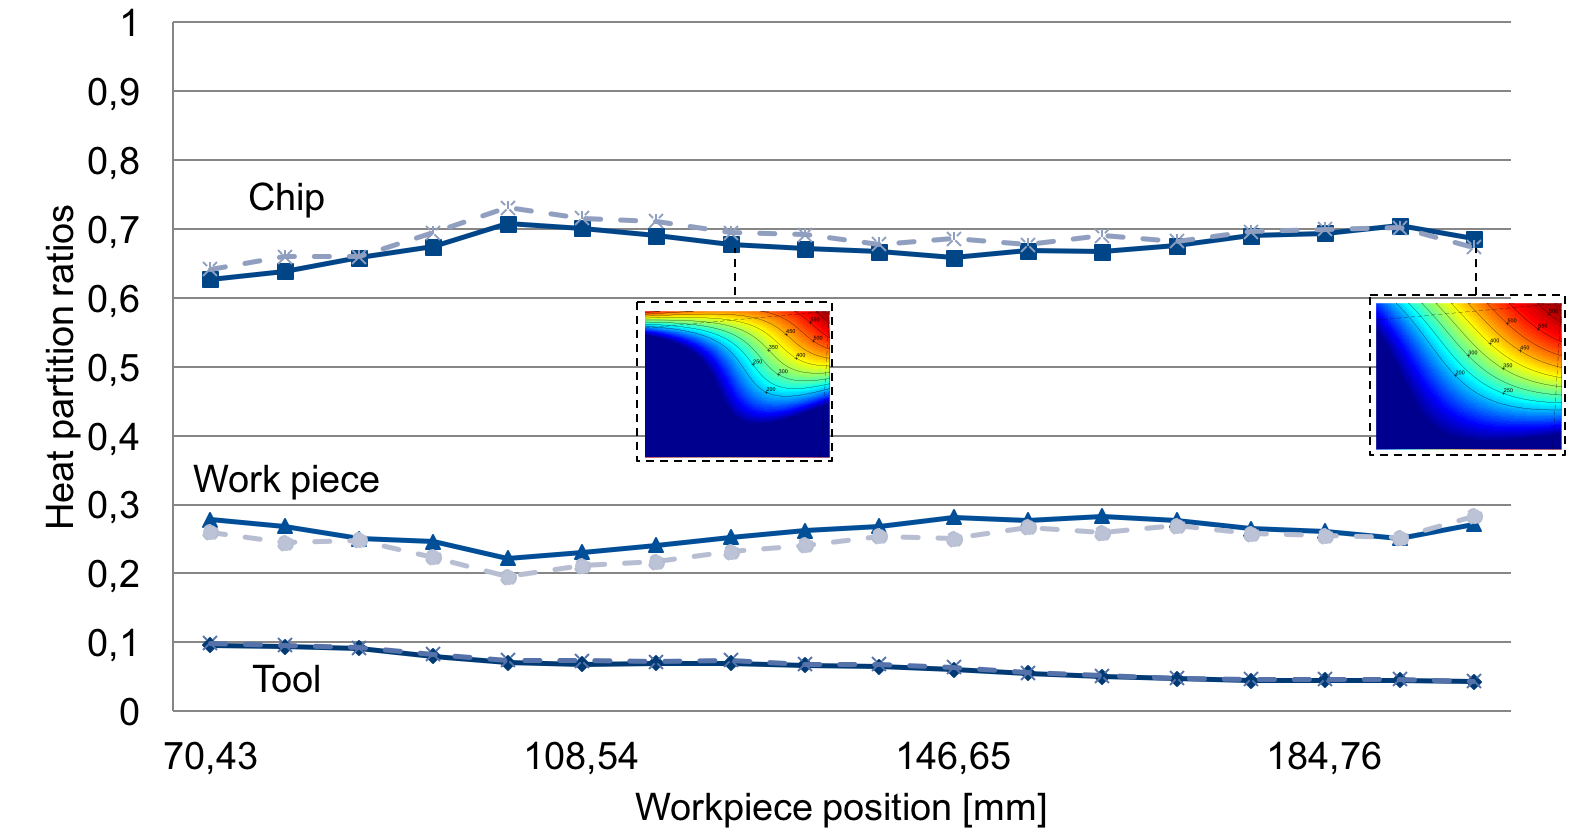
\includegraphics[scale=0.55]{Imagens/partition500150.png}
			\caption{Heat partition for experiment with a$_{p}$ = 500$\mu$m and v$_{c}$ = 150 m/min}
			\label{fig:hpartExp}
		\end{figure}